%
% chap001.tex
%

%======================================================
\newcommand{\cmd}[1]{%
  \fcbox{navajowhite}{\textsf{#1}}
}%

%======================================================
\chapter{GET Web Content}

%======================================================
\section{HTTP request using Node.js \& Javascript}
%======================================================
The only difference between \cmd{http.get} and
\cmd{http.request} is that \cmd{http.get}
automatically call the \cmd{http.request.end()} method.

\begin{lstlisting}

\begin{definition}[Primzahl]
``Eine Primzahl ist eine natürliche Zahl $p > 1$, die nur 
die trivialen Teiler besitzt, d.h. deren einzige Teiler
1 und sie selbst sind'' \cite{schichlsteinbauer}, S. 23.
\end{definition}
\vspace{-.5cm}

\begin{minipage}{0.65\linewidth}
Die Primzahlen sind nicht vor einer kurzen Zeit erfunden
worden. Schon vor mehrere hunderte von Jahren hatten sich
die Mathematiker mit den Primzahlen beschäftigt.
Hinsichtlich der Mathematiker, die als erste die Primzahlen
untersuchten, sind die Mathematiker der pythagoräischen
Schule (ab 500 bis 300 v. Chr.). Sie fokussierten sich auf
die perfekten und befreundeten Zahlen und infolgedessen
untersucheten sie die Primzahlen, aber auch die
zusammengesetzten Zahlen. Es wurden viele relevante
Entdeckungen von ihnen gemacht, jedoch konnten sie ihre
Theorien nicht beweisen.
\end{minipage}
\hfil
\begin{minipage}[r]{0.3\linewidth}
  % insert this 2 lines before \includegraphics to avoid the warning "the option `hypcap=true' will be ignored for this particular \caption on input line.
  % This warning occurs, because a conflict at paramter "hypcap=true" when load both packages "hyperref" and "caption".
  %\captionsetup[figure]{font=small,skip=6pt}%{labelformat=empty}% turn off figure prefix "Figure:" or "Abbildung"
  \captionsetup{type=figure,font=small,skip=6pt,format=plain}% {format=hand}
  \capstart
  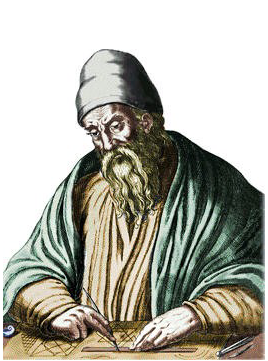
\includegraphics[width=1.0\linewidth]{./images/euklid.png}
  \captionof{figure}[Fantasieportrait Euklids. Das Bild wurde von Norbert Froese's Arbeit \textit{``Euklid und die Elemente. Die Entdeckung der axiomatischen Methode durch Euklid"} kopiert. Das ursprüngliche Bild stammt vom französischen Maler Charles Paul Landon (1760 – 1826). https://www.antike-griechische.de/Euklid.pdf. 2021)]{Euklid und die Elemente, 2021}
  \label{fig:portrait_euklid}
\end{minipage}
\vspace{.3cm}

``Um 300 v. Chr. veröffentlichte Euklid~\index{Euklid} die Bücher der
”Elemente“, die viele wichtige Erkenntnisse der
Primzahlforschung\index{Primzahl!Forschung}
mit korrekt geführten Beweisen beinhalteten'' (vgl. Sas
2002-2008, S. 4). Einer der wichtigen Beweise sind die
unendlich vielen Primzahlen.

\begin{theorem}[Satz von Euklid]
Es gibt unendlich viele Primzahlen.
\end{theorem}

\begin{proof}
(vgl. \cite{schichlsteinbauer}, S. 25).
\end{proof}

\newpage

%======================================================
\section{Primzahltests}
%======================================================

Wie im ersten Unterkapitel beschrieben, sind die Primzahlen
unendlich. Das heißt, dass es auch große Primzahlen
existieren, die für viele Verschlüsselungsverfahren immens
bedeutend sind.
